\documentclass[paper=a4, fontsize=11pt]{scrartcl}
\usepackage[T1]{fontenc}
\usepackage{fourier}

%\usepackage[english]{babel}															
\usepackage[english]{babel}
\usepackage{indentfirst}		% for indent
\usepackage[utf8]{inputenc}


\usepackage[protrusion=true,expansion=true]{microtype}	
\usepackage{amsmath,amsfonts,amsthm} % Math packages
\usepackage[pdftex]{graphicx}	
\usepackage{url, array}
\usepackage[num,abnt-repeated-author-omit=yes]{abntex2cite}


%%% Custom sectioning
\usepackage{sectsty}
\allsectionsfont{\centering \normalfont\scshape}


%%% Custom headers/footers (fancyhdr package)
\usepackage{fancyhdr}
\pagestyle{fancyplain}
\fancyhead{}											% No page header
\fancyfoot[L]{}											% Empty 
\fancyfoot[C]{}											% Empty
\fancyfoot[R]{\thepage}									% Pagenumbering
\renewcommand{\headrulewidth}{0pt}			% Remove header underlines
\renewcommand{\footrulewidth}{0pt}				% Remove footer underlines
\setlength{\headheight}{13.6pt}


%%% Equation and float numbering
\numberwithin{equation}{section}		% Equationnumbering: section.eq#
\numberwithin{figure}{section}			% Figurenumbering: section.fig#
\numberwithin{table}{section}				% Tablenumbering: section.tab#


%%% Maketitle metadata
\newcommand{\horrule}[1]{\rule{\linewidth}{#1}} 	% Horizontal rule

%\date{\today}

%%% Begin document
\begin{document}
		
{\flushleft\horrule{2pt}
\begin{center}
{
\includegraphics[height=0.09\textwidth]{Figs/logo_english.png}} 
\begin{tabular}{ m{1.8cm} m{10cm} m{1.8cm}}
\begin{center}
\end{center}
&
\begin{center} 
{\small
{Adrar University} \\
{Faculty of Science and Technology} \\
{Department of Mathematics and Computer Science}} \\

\end{center}
&

\begin{center}
\end{center}
\end{tabular}
\end{center}
\flushleft \horrule{2pt}\\[1cm]
}


\begin{center}

{
\huge  
Initiation to Research (Course) \\
\vspace{0.2cm}
2\textsuperscript{nd} Year Master (S3) \\
\vspace{0.2cm}
2020/2021}\\

\vspace{1cm}

{
\Huge   
\textbf{A hybrid meta-heuristic for better localization of nodes in RCSFs }}\\
\vspace{1cm}

%Domain: Mathematics and Computer Science \\
%Major: Informatics - Intelligent Systems \\
{
\Large
\textbf{BenSmail Moulay Ali cherif \footnote{Email: 	bensmail.moulayalicherif@gmail.com} \\ Lila Moatez \footnote{Email: dadalila194@gmail.com}}}\\
\vspace{3cm}

{
\large
\textbf{Instructor: Dr. Abdelghani DAHOU \footnote{Email: dahou.abdghani@univ-adrar.edu.dz}}}\\
\today
\end{center}
\pagebreak
\tableofcontents
\pagebreak
\listoffigures
\pagebreak
\listoftables
\pagebreak




\section{Introduction}
In the field of the wireless sensor network, more precisely the location of the sensor, when we disperse the sensors in an environment, in any application (agriculture, forest fires, military, medicine, security, etc.), it is necessary to know the location of the sensors, because without knowing the location of the sensor we cannot know where the event was captured, and to know the location, there are several methods, in particular meta-aristics.
     A meta-heuristic is an optimization algorithm aimed at solving difficult optimization problems. Usually iterative stochastic algorithms, which progress towards a global optimum, that is to say the global extremum of a function, by sampling an objective function.



.
.
\subsection{Statement of the Focus and Purpose of the Study}
\begin{itemize}
   Sensor networks have stimulated scientific and industrial societies, and they consist of a group of smart sensors capable of communicating with each other, whose mission is to collect and process information.
 It led to a great development in the medical, environmental, and military fields, etc.
 The areas of their use are clear, on the one hand, and on the other hand, cause several problems, and it is only responsible for receiving information from the middle and sending it from sensor to sensor until it reaches the main station.
\end{itemize}

\subsection{Research Questions/Hypotheses}
    Among the problems encountered: The problem of the location: It is represented in determining the geographic location of the sensor (real or estimated), for example, knowing the event will be useless if you do not know the location of its occurrence, for example: forest fires.
 This is why location is one of the main problems with this type of network.
GPS is the most used system around the world, but equipping all nodes in the network with GPS is very expensive, so we use positioning algorithms that depend on a group of well-known nodes called anchors.
     There are two methods, either estimating distances, we use technologies (RSSI, ToA, TDoA), and eager locations (Centroid, Dv hop), i.e.  Approximate location, depending on the extent of the sensed communication.

\subsection{Theory and Method/Methodology}
Briefly introduce your:

    In this thesis, a recently developed méta heuristic algorithm, called the FoA algorithm, is proposed, and it relies on the patterns and behavior of flash fireflies.
     We are improving this algorithm to reduce site error.
     And we compare it with other algorithms based on error and change their settings.


\section{Methodology/Research Methods}
used a MATLAB simulator for our simulation.
To carry out our work, we have organized it into four chapters as follows:
\begin{itemize}

    \item  Chapter 1: We present the state of the art on wireless sensor networks.
    \item Chapter 2: is devoted to study and bibliographic research of localization algorithms in wireless sensor networks. 
    \item Chapter 3: constitutes the heart of our work, in this chapter we present the application of matlab with a brief description of, validation and simulation of the FoA (firefly algorithm).  Subsequently we give the results in the form of graphs, and evaluation to see the precision of the method.

\end{itemize}
 We will end this brief with a general conclusion and summarize all the work.
\section{Project Timeline}
A description of your project's workflow and schedule, including the GANTT chart and its corresponding description.


\pagebreak

 \begin{figure}
    \centering
    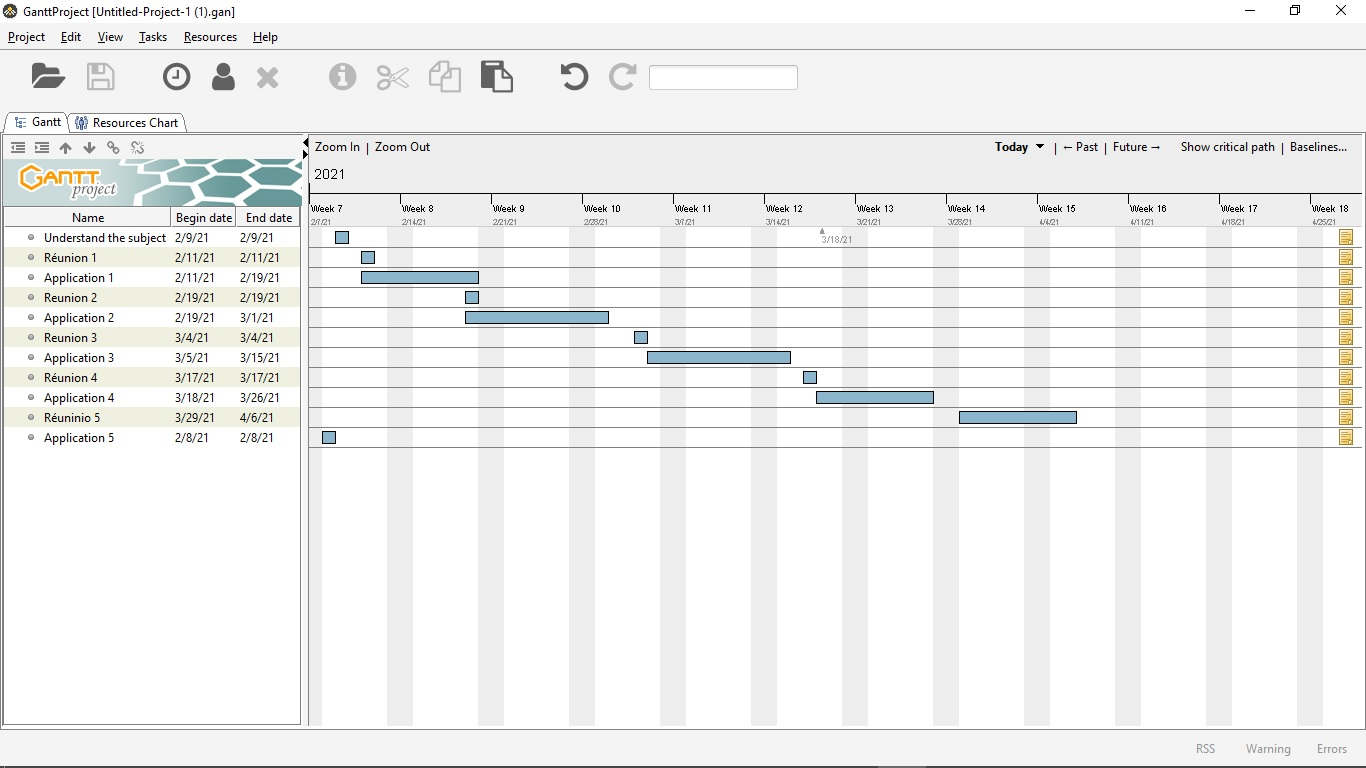
\includegraphics[height=0.55\textwidth]{Figs/GG.jpg}
    \caption{Project Time Line}
    \label{fig:my_label}
\end{figure}

\pagebreak
\bibliographystyle{abnt-num}
\bibliography{ref}

\end{document}